%%%%%%%%%%%%%%%%%%%%%%% file template.tex %%%%%%%%%%%%%%%%%%%%%%%%%
%
% This is a general template file for the LaTeX package SVJour3
% for Springer journals.          Springer Heidelberg 2010/09/16
%
% Copy it to a new file with a new name and use it as the basis
% for your article. Delete % signs as needed.
%
% This template includes a few options for different layouts and
% content for various journals. Please consult a previous issue of
% your journal as needed.
%
%%%%%%%%%%%%%%%%%%%%%%%%%%%%%%%%%%%%%%%%%%%%%%%%%%%%%%%%%%%%%%%%%%%
%
% First comes an example EPS file -- just ignore it and
% proceed on the \documentclass line
% your LaTeX will extract the file if required
\begin{filecontents*}{example.eps}
%!PS-Adobe-3.0 EPSF-3.0
%%BoundingBox: 19 19 221 221
%%CreationDate: Mon Sep 29 1997
%%Creator: programmed by hand (JK)
%%EndComments
gsave
newpath
  20 20 moveto
  20 220 lineto
  220 220 lineto
  220 20 lineto
closepath
2 setlinewidth
gsave
  .4 setgray fill
grestore
stroke
grestore
\end{filecontents*}
%
\RequirePackage{fix-cm}
%
%\documentclass{svjour3}                     % onecolumn (standard format)
%\documentclass[smallcondensed]{svjour3}     % onecolumn (ditto)
%\documentclass[smallextended]{svjour3}       % onecolumn (second format)
\documentclass[twocolumn]{svjour3}          % twocolumn
%
\smartqed  % flush right qed marks, e.g. at end of proof
%
\usepackage{graphicx}
%
% \usepackage{mathptmx}      % use Times fonts if available on your TeX system
%
% insert here the call for the packages your document requires
%\usepackage{latexsym}
% etc.
%
% please place your own definitions here and don't use \def but
% \newcommand{}{}
%
% Insert the name of "your journal" with
% \journalname{myjournal}
%
\begin{document}

\title{Multifractal characterization and classification of bread crumb digital images%\thanks{Grants or other notes
%about the article that should go on the front page should be
%placed here. General acknowledgments should be placed at the end of the article.}
}
%\subtitle{Do you have a subtitle?\\ If so, write it here}

%\titlerunning{Short form of title}        % if too long for running head

\author{Rodrigo Baravalle         \and
        Claudio Delrieux \and
        Juan Carlos G\'omez
}

%\authorrunning{Short form of author list} % if too long for running head

\institute{Rodrigo Baravalle and Juan Carlos G\'omez \at
              Laboratorio de Sistemas Din\'amicos y Procesamiento de Informaci\'on \\
              FCEIA, Universidad Nacional de Rosario, - CIFASIS - CONICET \\
              Riobamba 250 bis, 2000, Rosario, Argentina. \\
              Tel.: +54-341-4237248 int. 301\\
              Fax: +54-341-4821772 int. 3\\
              \email{baravalle@cifasis-conicet.gov.ar}
           \and
           Claudio Delrieux \at
               DIEC, Universidad Nacional del Sur - IIIE-CONICET \\
               Avenida Col\'on 80 - Bah\'ia Blanca (8000FTN) \\
               Provincia de Buenos Aires - Rep\'ublica Argentina
}

\date{Received: date / Accepted: date}
% The correct dates will be entered by the editor


\maketitle

\begin{abstract}
Adequate image descriptors are fundamental in image classification and object recognition. Main requirements for image features are robustness and low dimensionality which would lead to low classification errors in a variety of situations and with a reasonable computational cost.

In this context, the identification of materials poses a significant challenge, since typical (geometric and/or differential) feature extraction methods are not robust enough. Texture features based on Fourier or wavelet transforms, on the other hand, do withstand geometric and illumination variations, but tend to require a high amount of descriptors to perform adequately. 

Recently, the theory of fractal sets has shown to provide local image features that are both robust and low-dimensional. In this work we apply fractal and multifractal feature extraction techniques for bread crumb classification based on colour scans of slices of different bread types. Preliminary results show that fractal based classification is able to distinguish different bread crumbs with very high accuracy.
\keywords{Fractal \and Multifractal \and Classification \and Bread crumb}
% \PACS{PACS code1 \and PACS code2 \and more}
% \subclass{MSC code1 \and MSC code2 \and more}
\end{abstract}

\section{Introduction}
\label{intro}
Fractal and multifractal analysis of images have proved to capture useful properties of the underlying material being represented. Characterisation of images using these features have been successfully applied in different areas, such as medicine (\cite{Andjelkovic2008,Yu2011}) and texture classification (\cite{Wendt2009}). Through several procedures, it is possible to obtain different Fractal Dimensions (FD), each of them capturing a different property of the material ({\em e.g.}, void image fraction, rugosity).

For each material, the results obtained in the classification process are useful in quality measurements of real samples and also in the validation of synthetic representations of them. In other words, the classification is useful to determine if a given image presents the observed features in that material, allowing to associate quality measure parameters to the material. In~\cite{Fan2006}, a quality bread crumb test based on Gabor filters was performed in that paper, obtaining good results. Nevertheless, a small database was used ($30$ images). In \cite{Gonzales2008} several fractal features were obtained for one type of bread, showing that a vector comprising them would be capable of obtaining key features of its crumb texture.

In this work we propose the application of the MFS \cite{XX} to describe and discriminate among different bread types. **ILLUMINATION INVARIANCE**

 fractal and multifractal descriptors for the classification of different bread types and for the discrimination between bread and non-bread images. The proposed method is compared to a classifier that uses only mean colour information. The results of this feature extraction procedure show that the classifier is robust and presents good discrimination properties to distinguish between different types of bread and also non bread images. In section 2 we briefly introduce the theory underlying fractal sets. In section 3 we describe the materials and methods employed in the classification. In section 4 we show the results obtained in the classification and we perform a robustness analysis of the method. In section 5 we summarise the conclusions, and we pose some possible future works.

\section{Materials and Methods}
\label{sec:1}
\subsection{Fractals and Multifractals}
\label{sec:2}
as required. Don't forget to give each section
and subsection a unique label (see Sect.~\ref{sec:1}).
\paragraph{Paragraph headings} Use paragraph headings as needed.
\begin{equation}
a^2+b^2=c^2
\end{equation}

% For one-column wide figures use
%\begin{figure}
% Use the relevant command to insert your figure file.
% For example, with the graphicx package use
%  \includegraphics{example.eps}
% figure caption is below the figure
%\caption{Please write your figure caption here}
%\label{fig:1}       % Give a unique label
%\end{figure}
%
% For two-column wide figures use
%\begin{figure*}
% Use the relevant command to insert your figure file.
% For example, with the graphicx package use
%  \includegraphics[width=0.75\textwidth]{example.eps}
% figure caption is below the figure
%\caption{Please write your figure caption here}
%\label{fig:2}       % Give a unique label
%\end{figure*}
%
% For tables use
%\begin{table}
% table caption is above the table
%\caption{Please write your table caption here}
%\label{tab:1}       % Give a unique label
% For LaTeX tables use
%\begin{tabular}{lll}
%\hline\noalign{\smallskip}
%first & second & third  \\
%\noalign{\smallskip}\hline\noalign{\smallskip}
%number & number & number \\
%number & number & number \\
%\noalign{\smallskip}\hline
%\end{tabular}
%\end{table}

\subsection{Box dimension}
\label{sec:3}
Box FD is a simplification of the Hausdorff (originally Minkowski - Bouligand) dimension for non strictly self-similar objects (\cite{Peitgen2004}). Given a binarised image, it is subdivided in a grid of size $M\times M$ where the side of each box formed is $\epsilon$. If $N_{\epsilon}$ represents the amount of boxes that contains at least one pixel in the binarisation of the set for that $\epsilon$, then the box dimension  $D_{b}$ is defined as

\begin{equation}
D_{b} \triangleq \displaystyle\lim_{\epsilon \to 0}{\frac{\log(N_{\epsilon})}{\log (1/\epsilon)}}.
\label{eqn:1}
\end{equation}

The algorithm computes a binarised image from the original one and then selects different values of $\epsilon$ in it, making a count of the boxes that contains pixels in each case (to avoid numerical instabilities, a mean of cases is computed, establishing different positions in the grid over the image). Finally, a linear regression adjustment is made with the obtained data, in the $\log-\log$ space, and the slope of the straight line is by definition the box dimension of the image. %In Fig. \ref{fig:1} an image of the bread type {\em salvado} is shown with its corresponding box dimension computation.


\subsection{Multifractal analysis}
\label{sec:4}
Some elements in nature show fractal features or auto similarity. The fractal dimension is an exponent which relates the statistical auto similarity of the object at different scales. On the one hand, deterministic fractals are characterized by the same FD at all scales. They are called {\em monofractals} (for instance, Koch Curve, Sierpinsky triangle). On the other hand, {\em multifractals} (\cite{Mandelbrot89}) are characterized by a set of FDs depending on the scale. It is assumed that these structures are composed by different fractals coexisting simultaneously.

\subsubsection{H\"older exponent}
\label{sec:5}
Informally, the way to proceed with multifractal analysis is to examine, in the limit, the local behaviour of a measure $\mu$ at each point of the set under study. This means, to find the H\"older exponent $\alpha$ in that point. The {\em multifractal spectrum} $f(\alpha)$ is obtained applying this procedure to the entire set, in this case, an image.

Let $E$ be an structure divided in disjoint substructures $E_{i}$ of size $\epsilon$ in such a way that 

\begin{equation}
\displaystyle\bigcup_{i}E_{i} = E.
\end{equation}

Each substructure $E_{i}$ is characterized by a measure $\mu(E_{i})$. From the point of view of multifractal analysis, it is useful to define this value as a function of $\epsilon$, {\em i.e.}


\begin{equation}
\alpha_{i} = \frac{ln(\mu(E_{i}))}{ln(\epsilon)},
\label{eqn:eqn4}
\end{equation}
\noindent
and to take the limit when $\epsilon$ tends to $0$. The limit represents the value of the H\"older exponent at a point in the structure, that is

\begin{equation}
\alpha = \lim_{\epsilon\to0}{\alpha_{i}}.
\label{eqn:eqn5}
\end{equation}

The exponent characterizes the local regularity of the structure at a point. To obtain a global characterization of its regularity it is necessary to obtain the distribution of $\alpha$ in $E$. For this, a counting $N_{\epsilon}$ must be done for each $\alpha_{i}$, related to the value of $\epsilon$, {\em i.e.}

\begin{equation}
f_{\epsilon}(\alpha_{i}) = - \frac{ln(N_{\epsilon}(\alpha_{i}))}{ln(\epsilon)}.
\label{eqn:eqn6}
\end{equation}

When $\epsilon$ tends to $0$, the limiting value is the FD of the structure $E$ characterized by $\alpha$, the Hausdorff dimension of the $\alpha$ distribution, also known as the {\em multifractal spectrum} $f(\alpha)$ (\cite{Silvetti2010}), {\em i.e.}

\begin{equation}
f(\alpha) = \lim_{\epsilon\to0}{f_{\epsilon}(\alpha)}.
\label{eqn:eqn7}
\end{equation}

\subsubsection{Procedure for the MFS}
As illustrated in \cite[XuXXX], the domain is partitioned into non-overlapping boxes of length $r$. The $q$-th moment of a measure $\mu$ is defined as
\begin{equation}
M_{r}(q) = \sum{\mu(B(x,r))^{q}},
\label{eqn:eqn8}
\end{equation}

where the sum is over the $r$ mesh squares for which $\mu(B(x,r)) > 0$. To denote the power law behavior of $M_{r}(q)$, $\beta(q)$ is defined as a line fitting of the values $M_{r}(q)$ with respect to $r$, for $r in 1,..,n$. It is shown in \cite[FalconerXXX], that the MFS and $\beta(q)$ are related to each other by a Legendre transform as

\begin{equation}
f(\alpha(q)) = q \alpha(q) - \beta(q),
\label{eqn:eqn9}
\end{equation}

where

\begin{equation}
\alpha(q) = \frac{d\beta(q)}{dq}.
\label{eqn:eqn10}
\end{equation}

Using equations \ref{eqn:eqn7} and \ref{eqn:eqn8} the MFS is estimated. In this paper, the author's implementation is used.

The first approach is to define $\mu$ in the intensity domain, {\em i.e.}

\begin{equation}
\mu(B(x,r)) = \int_{B(x,r)}{(G_{r} \ast I)} dx,
\label{eqn:eqn11}
\end{equation}

where $\ast$ is the $2D$ convolution opeartor and $G_{r}$ is a Gaussian smoothing kernel with variance $r$, {\em i.e., } $\mu$ is the average intensity value in the disk of radius $r$ centred at $x$ ($B(x,r)$). This is the density of the intensity function, and it describes how the intensity at a point changes over scale.

\subsection{Image acquisition}
\label{sec:7}
%(in the case of baguette and salvado, since the two other types were already sliced in the moment of purchase).
$20$ images of four different bread types ({\em lactal}, {\em baguette}, {\em salvado} and {\em sandwich}), counting $80$ images, were obtained using an electric slicer. The images were digitalised using an HP PSC 1210 scanner and they were saved in TIFF format. Images showed a resolution of $380 \times 380$ pixels (the maximum possible area for the four bread types) and $350$ dpi ($1$ pixel $= 0.00527 mm^{2}$). Then the images were converted to grey scale ($8$ bits). In addition, $20$ images of each bread type were acquired with a digital camera, using the same spatial resolution, counting $80$ images. The illumination conditions of these images were different from that of the scanner in order to test for the robustness of the method. In Fig.~\ref{fig:camera} four examples of bread images from the camera are shown. We also employed one hundred randomly selected images from the CalTech101~(\cite{FeiFei04}) dataset in order to test the method's performance with non-bread images. In Fig.~\ref{fig:nonbread} four examples of non-bread images from this dataset are shown. 

To calculate the void fraction, mean cell area and standard deviation of mean cell area, the image should be binarized. The algorithm presented in \cite{White83} was used. This algorithm applies a local thresholding schema, which showed better results than using a global thresholding schema. Particularly, the algorithm presented in \cite{Huang95} and used in \cite{Gonzales2008}, showed poor results when the illumination conditions vary in the image. In Fig.~\ref{fig:bread} an image of each bread type used in this work (top row) and its resulting binarisation using the proposed algorithm (bottom row) is shown. Small elements of one and two pixels were eliminated by an opening operation (erosion and dilation) using a $2\times2$ structuring element. The method showed good results even for different illumination conditions varying in the image. 

In order to determine the result of the binarization at a pixel, the algorithm obtains some average from the gray level in a window surrounding the pixel, and compares it to a threshold determined by the actual gray level of the pixel and a bias which is multiplied by this value. Two parameters must be set in the algorithm: the size of the window and the bias. It was found that different values are needed for better results when different capturing methods are used. The values for the scanner samples were $80$ for the window and $1.15$ for the bias. In the case of digital camera samples, the values found were $100$ and $1$ for the bias. These differences appears due to the different illumination conditions present in the images resulting from these different capturing conditions. Further research is required in order to determine automatic values for these parameters.

\begin{figure*}[htb]
\centering
\includegraphics[scale=1.3]{imagenes/baguette20}
\includegraphics[scale=1.3]{imagenes/lactal14}
\includegraphics[scale=1.3]{imagenes/salvado43}
\includegraphics[scale=1.3]{imagenes/sandwich43}
%includegraphics[scale=0.265]{imagenes/baguette20bin}
%\includegraphics[scale=0.333]{imagenes/lactal14bin}
%\includegraphics[scale=0.333]{imagenes/salvado43bin}
%\includegraphics[scale=0.333]{imagenes/sandwich43bin}
\caption{Digitalised images of {\em baguette}, {\em lactal}, {\em salvado} and {\em sandwich} bread types}
\label{fig:bread}
\end{figure*}

\begin{figure*}[htb]
\centering
\includegraphics[scale=0.28]{imagenes/caltech/image_0066}
\includegraphics[scale=0.28]{imagenes/caltech/image_0083}
\includegraphics[scale=0.28]{imagenes/caltech/image_0284}
\includegraphics[scale=0.28]{imagenes/caltech/image_0300}
\caption{Images from the dataset CalTech101}
\label{fig:nonbread}
\end{figure*}

\begin{figure*}[htb]
\centering
\includegraphics[scale=0.28]{imagenes/camera/b}
\includegraphics[scale=0.28]{imagenes/camera/l19}
\includegraphics[scale=0.28]{imagenes/camera/s7}
\includegraphics[scale=0.28]{imagenes/camera/Sa14}
\caption{Digitalised images from a digital camera}
\label{fig:camera}
\end{figure*}

\subsection{Feature vectors}
\label{sec:8}
Following the ideas presented in \cite{Gonzales2008}, the mentioned fractal and multifractal features were obtained for each image (using $20$ H\"older exponents). For each image, a $42$-dimensional feature vector was computed. The code of the algorithms for the computation of the Box dimension, the Morphological fractal dimension and the multifractal spectrum were written and run in Matlab. In order to make a comparison, a $3$-dimensional feature vector, with RGB colour features was also computed (R mean, G mean, B mean).

Self-organizing maps (SOM)~(\cite{Kohonen2001}) of the vectorized images are useful to visualize these different representation of bread images into a lower dimensional view, in order to understand them better. A SOM maps high dimensional data into a (typically) two-dimensional representation, using neighbourhood information. Topological information of the original data is preserved.  

Unsupervised SOM of the fractal and non fractal representations of scanned images are shown in Fig.~\ref{fig:somfractal} and Fig.~\ref{fig:somrgb} respectively. The fractal features SOM seems to show easily separable classes while the RGB features SOM appears to be more overlapped. It seems that a classifier could potentially obtain better classification results using the fractal features. %%Next sections will show that this hypothesis is true.
%Also, in the latter, the non bread class seems to be spread over the rest of the classes, making it more difficult to distinguish between bread and non bread images. 

%\begin{figure*}

%\begin{centering}
%\subfloat[Fractal features SOM]{\begin{centering}
%\includegraphics[width=0.6\textwidth]{exps/som/som\mydot multifractal}
%\label{fig:somfractal}
%\par\end{centering}
%}

\section{Results}
\label{sec:9}
\subsection{Bread Classification}
\label{sec:10}
Experiment explanation...

\begin{table}
% table caption is above the table
\caption{Intra-class classification results for the bread crumb database}
\label{tab:1}       % Give a unique label
% For LaTeX tables use
\begin{tabular}{lllll}
\hline\noalign{\smallskip}
Classifier & MFS (20) & MFS+L (20) & MFS+G (20) & SIFT  \\
\noalign{\smallskip}\hline\noalign{\smallskip}
SVM & 94.5 & 95.5 & 97.5 & 96.5 \\
RF  & 93.5 & 96 & 95 & 92 \\
NN & 90.5 & 90 & 87 & 86 \\
\noalign{\smallskip}\hline
\end{tabular}
\end{table}


\begin{table}
% table caption is above the table
\caption{classification results with different number of FDs for the MFS}
\label{tab:2}       % Give a unique label
% For LaTeX tables use
\begin{tabular}{lllll}
\hline\noalign{\smallskip}
 & 10  & 20 & 30 \\
\noalign{\smallskip}\hline\noalign{\smallskip}
SVM & 96 & 94.5 & 95.5 \\
RF  & 91.5 & 93.5 & 93 \\
NN & 88.5 & 90.5 & 90 \\
\noalign{\smallskip}\hline
\end{tabular}
\end{table}

\begin{table}
% table caption is above the table
\caption{Intra-class classification results for different methods}
\label{tab:1}       % Give a unique label
% For LaTeX tables use
\begin{tabular}{llllll}
\hline\noalign{\smallskip}
Classifier & Haralick & Lbp & CIELab (L) & CIELab (L+a+b)\\ % & Zernicke
\noalign{\smallskip}\hline\noalign{\smallskip}
SVM & 94 & 78.5 & 94.0 & 97.5 \\ % & 55 
RF  & 91 & 71.5 & 93.5 & 96.0 \\ % & 58 
NN & 79 & 70 & 86 & 92.0 \\ % & 48.5 
\noalign{\smallskip}\hline
\end{tabular}
\end{table}


\subsection{Bread Classification}
\label{sec:10}
In Figure \ref{fig:meansMFS}, the mean values for the MFS, using $20$ FDs, for the four different bread types are shown.

\begin{figure*}[htb]
\centering
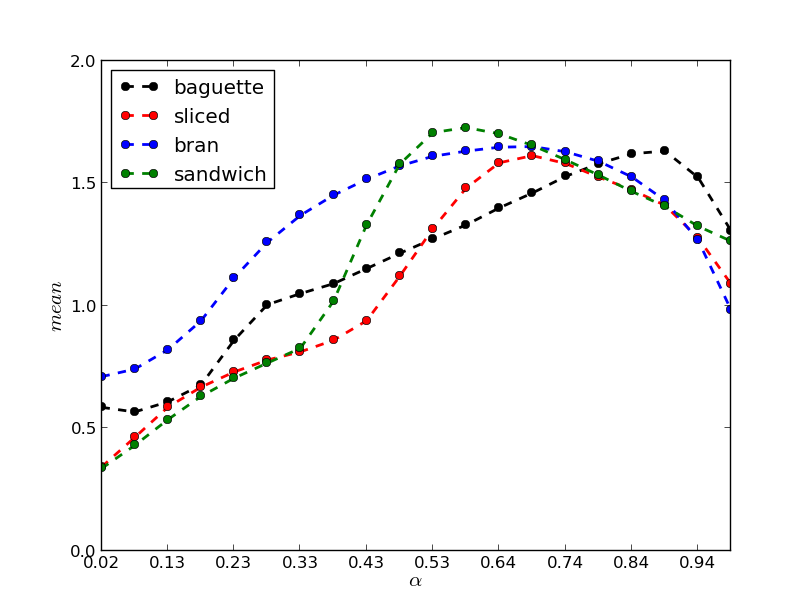
\includegraphics[scale=0.28]{../images/means}
\caption{Mean MFS for the four different types}
\label{fig:meansMFS}
\end{figure*}

The image shows...

The standard deviations for the four different bread types are shown in Table \ref{tab:4}. 



%\par\end{centering}

%\begin{centering}
%\subfloat[SOM using RGB features]{\begin{centering}
%\includegraphics[width=0.6\textwidth]{exps/som/som\mydot rgb}
%\label{fig:somrgb}
%\par\end{centering}
}
%\par\end{centering}

%\caption{SOM of the scanned bread images (classes $1$~--~$4$) and the non bread images (class $5$)}

%\end{figure*}

\section{Discussion}
\label{sec:11}
***CIELab
***VF, MCA, stCA

\section{Conclusions}
\label{sec:12}
The use of multifractal features in bread crumb texture classification showed good performance. The multifractal spectrum demonstrated to be accurate enough to perform a classification of different bread types and also to discriminate non bread from bread images. The use of non-fractal features such as colour, also showed comparable results, but it fails to detect non bread images, and it is easy to deceive it with false images. The combination of both classifiers showed similar results to those obtained using the fractal features, so the use of the latter alone is preferred. The three classifiers showed to be sensitive to illumination changes, making them still non robust. Preliminary tests on our particle system~(\cite{Baravalle2011}) show that it could deceive the fractal classifier, so further analysis is required in order to find the parameters that produce textures with similar fractal and multifractal features to those of real breads.

The results found can be applied to validate synthetic samples, {\em i.e.}, the latter should have similar features to the bread type that is trying to simulate. The features obtained will be used to determine particle system parameters ({\em e.g.}, lifetime of particles, colour). These results can be extended to be used as quality parameters for these products. The robustness of the method needs to be enhanced. Other FDs will be studied in order to accomplish this goal. Also, the code of the multifractal spectrum algorithm needs to be optimized in order to obtain a faster algorithm for bread classification. It will be useful to apply a Principal Component Analysis in order to identify the key variables in the feature vectors. 
%\begin{figure*}[htb]
%\centering
%$\vcenter{\hbox{\includegraphics[scale=1.3]{imagenes/salvado19}}}$
%$\vcenter{\hbox{\includegraphics[scale=0.4]{imagenes/fitbox}}}$
%\caption{An image and its computed box dimension}
%\label{fig:1}
%\end{figure*}

%\begin{acknowledgements}
%If you'd like to thank anyone, place your comments here
%and remove the percent signs.
%\end{acknowledgements}

% BibTeX users please use one of
%\bibliographystyle{spbasic}      % basic style, author-year citations
%\bibliographystyle{spmpsci}      % mathematics and physical sciences
\bibliographystyle{spphys}       % APS-like style for physics
\bibliography{bibliografia/bibliografia}   % name your BibTeX data base

% Non-BibTeX users please use
%\begin{thebibliography}{}
%
% and use \bibitem to create references. Consult the Instructions
% for authors for reference list style.
%
%\bibitem{RefJ}
% Format for Journal Reference
%Author, Article title, Journal, Volume, page numbers (year)
% Format for books
%\bibitem{RefB}
%Author, Book title, page numbers. Publisher, place (year)
% etc
%\end{thebibliography}

\end{document}
% end of file template.tex

